\section{Syntax analysis and parsing}

Consider the grammar $G$ below, represented as a machine net, over a three-letter terminal alphabet $\Sigma=\{a,b,c\}$ and a one-letter non-terminal alphabet (axiom $S$):
\begin{figure}[H]
    \centering
    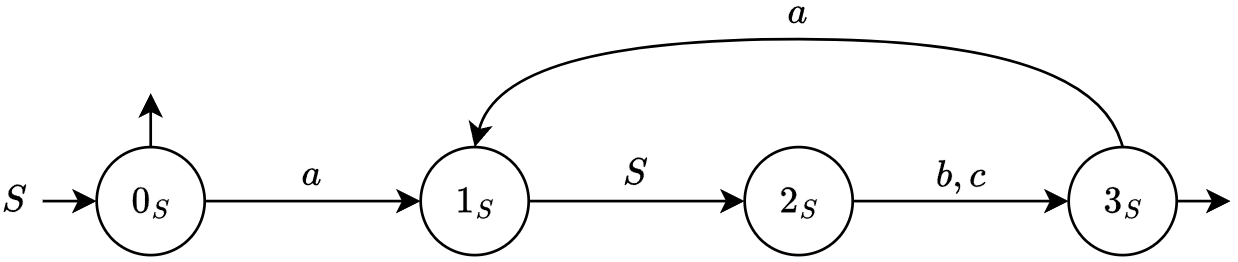
\includegraphics[width=0.5\linewidth]{images/mnet.png}
\end{figure}
Draw the complete pilot of grammar $G$, check for the conflicts, and show that grammar $G$ is ELR(1).

\paragraph*{Solution}
The initial state mirrors the one depicted in the provided machine. 
The final states are denoted by a circled name. 
The machine is illustrated below:
\begin{figure}[H]
    \centering
    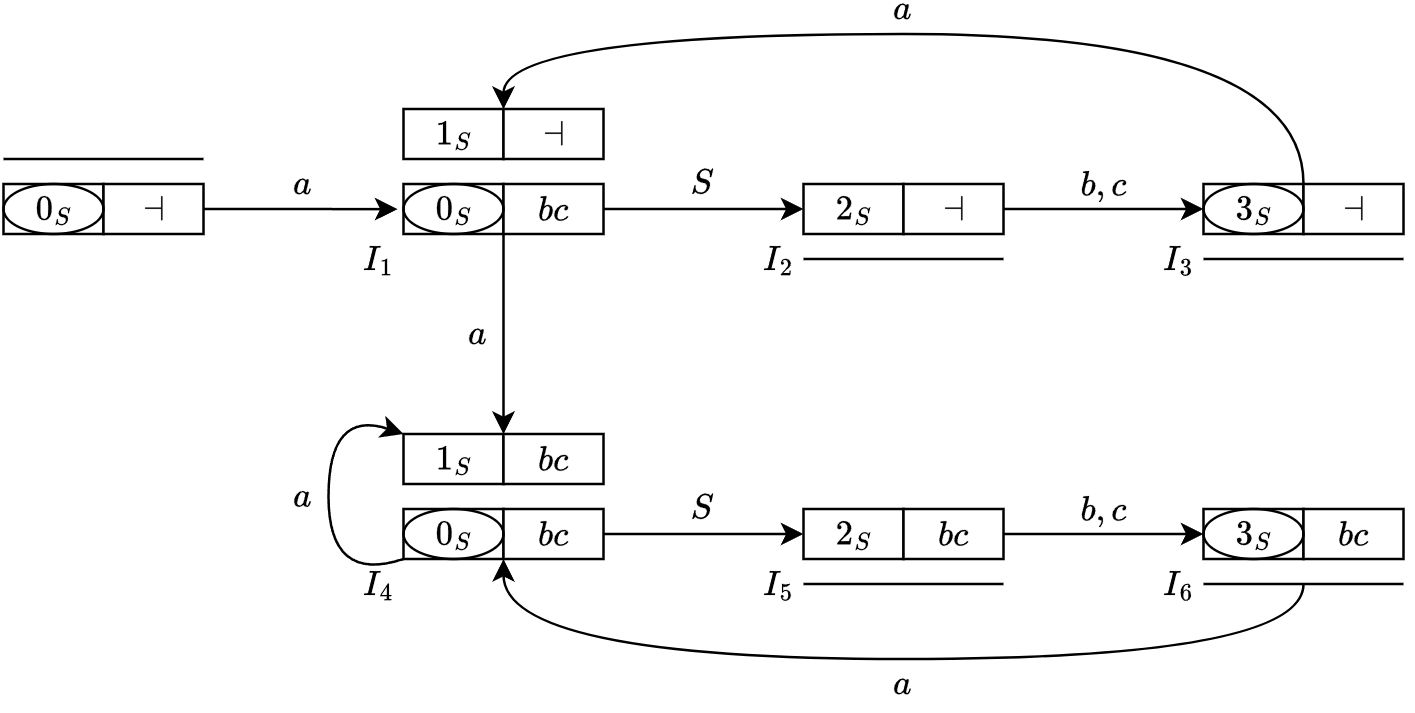
\includegraphics[width=0.75\linewidth]{images/pilot.png}
\end{figure} 
The shift/reduce conflicts are present if an outgoing arc from the terminal states has a label with a symbol in the look ahead of the terminal states. 
In this case we have no shift/reduce conflicts. 

The reduce/reduce conflicts are present if an $m$-state have two final states and at least one shared symbol in the two look ahead of the final state. 
In this case we have no reduce/reduce conflicts. 

Convergence conflicts manifest under the following conditions:
\begin{itemize}
    \item Loss of the single arc properties (non-determinism).
    \item Presence of two incoming arcs in an $m$-state with identical labels.
    \item Existence of a shared look ahead in the convergent $m$-states.
\end{itemize}
In this case we have no convergence conflicts. 

Given the absence of conflicts, it is evident that the grammar adheres to the ELR(1) property.